\documentclass[12pt]{article}
\usepackage{graphicx}
\usepackage[none]{hyphenat}
\usepackage{graphicx}
\usepackage{listings}
\usepackage[english]{babel}
\usepackage{graphicx}
\usepackage{caption} 
\usepackage{booktabs}
\usepackage{array}
\usepackage{amssymb} % for \because
\usepackage{amsmath}   % for having text in math mode
\usepackage{extarrows} % for Row operations arrows
\usepackage{listings}
\usepackage[utf8]{inputenc}
\lstset{
  frame=single,
  breaklines=true
}
\usepackage{hyperref}
  
%Following 2 lines were added to remove the blank page at the beginning
\usepackage{atbegshi}% http://ctan.org/pkg/atbegshi
\AtBeginDocument{\AtBeginShipoutNext{\AtBeginShipoutDiscard}}


%New macro definitions
\newcommand{\mydet}[1]{\ensuremath{\begin{vmatrix}#1\end{vmatrix}}}
\providecommand{\brak}[1]{\ensuremath{\left(#1\right)}}
\newcommand{\solution}{\noindent \textbf{Solution: }}
\newcommand{\myvec}[1]{\ensuremath{\begin{pmatrix}#1\end{pmatrix}}}
\providecommand{\norm}[1]{\left\lVert#1\right\rVert}
\providecommand{\abs}[1]{\left\vert#1\right\vert}
\let\vec\mathbf

\begin{document}

\begin{center}
\title{\textbf{VECTORS}}
\date{\vspace{-5ex}} %Not to print date automatically
\maketitle
\end{center}

\section{10$^{th}$ Maths - EXERCISE-7.3}

\begin{enumerate}
\item That a median of a triangle divides it into two triangles  of equal areas. verify this result for $\triangle ABC$ whose vertices are $\vec{A}(4,-6),\vec{B}(3,-2)\text{ and }\vec{C}(5,2)$.
\end{enumerate}

\section{SOLUTION}
Given points are
\begin{align}
\vec{A}=\myvec{4\\ -6} ,
\vec{B}=\myvec{3\\ -2} ,
\vec{C}=\myvec{5\\ 2}
\end{align}

Find the value
\begin{align}
\vec{D}&=\frac{\vec{B}+\vec{C}}{2}\\
&=\frac{\myvec{3\\ -2}+\myvec{5\\ 2}}{2}\\
&=\frac{\myvec{8\\ 0}}{2}\\
&=\myvec{4\\ 0}
\end{align}
Find the value of ar(ABC)
\begin{align}
ar(ABD)&=\frac{1}{2}\begin{vmatrix}
4 &3 &4 &4 \\
-6 &-2 &0 &-6
\end{vmatrix}\\
ar(ABC)&=3
\end{align}
Find the value of ar(ACD)
\begin{align}
ar ACD&=\frac{1}{2}\begin{vmatrix}
4 &5 &4 &4 \\
-6 &2 &0 &-6
\end{vmatrix}\\
ar(ACD)&=3
\end{align}
The median of the triangle is  both side areas are equal $\triangle ABD=\triangle ACD$
\begin{figure}[h]
\centering
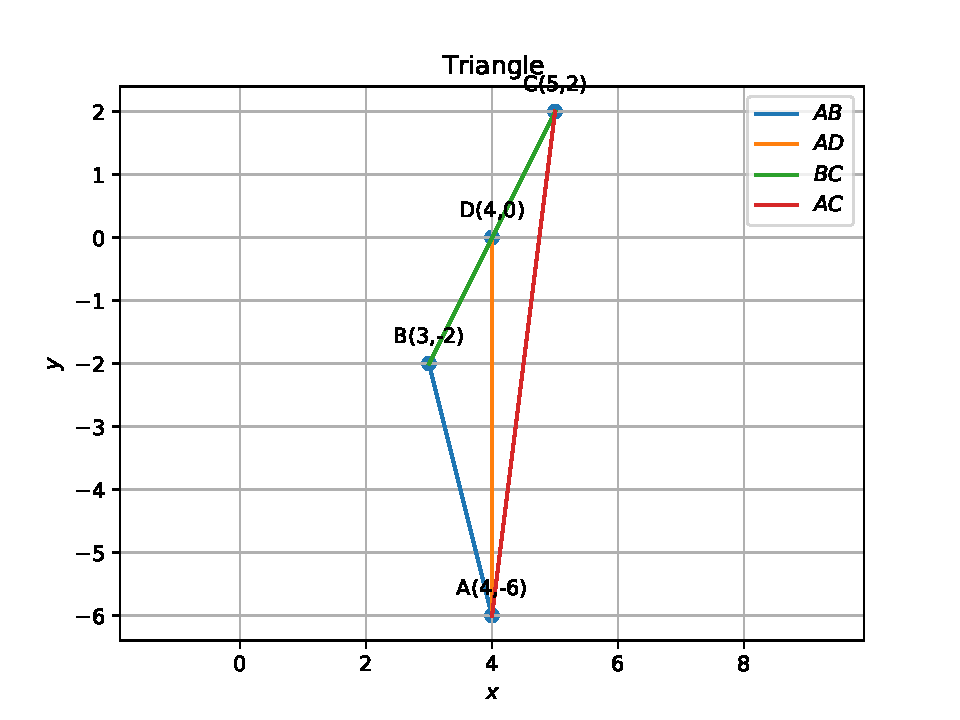
\includegraphics[width=\columnwidth]{fig.pdf}
\caption{Triangle}
\label{fig-}
\end{figure} 
\end{document}